\section{Difference in Threshold and Tolerance}
The mean for the three measurements of the threshold and tolerance before and after and the difference between these values for the treatment group and control group are illustrated in  \tabref{tab:Treatment} and \tabref{tab:Control} respectively. The standard deviation for these values are illustrated in \tabref{tab:TreatmentA} and \tabref{tab:ControlA} in \autoref{sec:ThresTolA}. The tolerance for some of the subjects are not representative, as the examiner was not able to apply enough force with the algometer. 

\begin{longtable} {l|c|c|c|c|c|c}
 \rowcolor[HTML]{C0C0C0} 
  \color[HTML]{000000}{} & 
 \multicolumn{3}{c|}{ \color[HTML]{000000}{\textbf{Threshold}}} & \multicolumn{3}{c}{ \color[HTML]{000000}{\textbf{Tolerance}}}  	\\  \rule{0pt}{3ex} 
  \cellcolor[HTML]{C0C0C0}{} &
 \multicolumn{1}{c|}{ \cellcolor[HTML]{C0C0C0}{Pre [KgF]}} & \multicolumn{1}{c|}{ \cellcolor[HTML]{C0C0C0}{Post [KgF]}} 
 & \multicolumn{1}{c}{ \cellcolor[HTML]{C0C0C0}{\textcolor[HTML]{C0C0C0}{0}Diff [\%]\textcolor[HTML]{C0C0C0}{0}}}
 & \multicolumn{1}{|c|}{ \cellcolor[HTML]{C0C0C0}{Pre [KgF]}} 
 & \multicolumn{1}{c|}{ \cellcolor[HTML]{C0C0C0}{Post [KgF]}} 
 & \multicolumn{1}{c}{ \cellcolor[HTML]{C0C0C0}{\textcolor[HTML]{C0C0C0}{0}Diff [\%]\textcolor[HTML]{C0C0C0}{0}}}  	\\ \hline 
\#T1 & 1.84 & 1.53 & -17.03 & 4.21 & 3.93 & -6.66 \\ \hline
\#T2 & 2.95 & 2.85  & -3.50 & 7.63  & 5.70 & -25.26 \\ \hline
\#T3 & 2.13 & 3.07 & 43.75 & 7.75 & 8.13 & 4.99 \\ \hline
\#T4 & 0.94 & 2.34  & 148.94  & 3.85 & 4.95 & 28.55 \\ \hline
\#T5 & 1.35 & 1.71  & 26.11 & 3.11 & 3.94 & 26.55 \\ \hline	
\#T6 & 0.31 & 0.94   & 206.52 & 5.95 & 5.99 & 0.67 \\ \hline
\#T7 & 2.07 & 2.74  & 32.15 & 5.44 & 8.82 & 62.13 \\ \hline
\#T8 & 1.82 & 3.59 & 97.44 & 7.21 & 10.11 & 40.11 \\ \hline
\#T9 & 2.17 & 2.84  & 31.08 & 6.98 & 9.62 & 37.82 \\ \hline
\#T10 & 4.71 & 4.85  & 3.12 & 12.37*  & 13.24* & 7.06 \\ \hline
\#T11 & 2.22 & 4.31 & 93.99 & 4.45 & 7.76 & 74.25 \\ \hline
\#T12 & 1.99 & 2.51 & 26.51 & 4.45 & 4.79 & 7.49 \\ \hline
\#T13 & 1.14 & 2.37 & 108.19 & 4.48 & 6.57 & 46.58 \\ \hline
\#T14 & 1.69 & 1.01 & -40.55 & 6.04 & 3.93 & -34.88 \\ \hline
\#T15 & 2.03 & 2.58 & 27.30 & 8.57* & 14.28* & 66.56 \\ \hline
\#T16 & 2.79 & 2.39 & -14.32 & 13.35* & 13.59* & 1.80 \\ \hline
\#T17 & 3.24 & 2.76 & -14.81 & 11.75 & 11.77* & 0.11 \\ \hline
\#T18 & 2.16 & 1.98 & -8.33 & 8.38* & 11.93* & 42.32 \\ \hline
\#T19 & 1.77 & 2.10 & 18.42 & 9.66 & 10.91 & 12.87  \\ \hline
\#T20 & 2.28 & 3.35 & 46.78 & 7.20  & 14.01* & 94.54 \\ \hline
\#T21 & 3.91 &  3.82 & -2.22 & 7.18 & 10.58 & 47.35 \\ \hline
	\caption{Threshold and tolerance before and after and the percentage difference between these values for the treatment group. The asterisk indicated that the tolerance was not representative.}
	\label{tab:Treatment}
\end{longtable}
\vspace{-.5cm}

\begin{longtable} {l|c|c|c|c|c|c}
 \rowcolor[HTML]{C0C0C0} 
  \color[HTML]{000000}{} & 
 \multicolumn{3}{c|}{ \color[HTML]{000000}{\textbf{Threshold}}} & \multicolumn{3}{c}{ \color[HTML]{000000}{\textbf{Tolerance}}}  	\\  \rule{0pt}{3ex} 
  \cellcolor[HTML]{C0C0C0}{} &
 \multicolumn{1}{c|}{ \cellcolor[HTML]{C0C0C0}{Pre [KgF]}} & \multicolumn{1}{c|}{ \cellcolor[HTML]{C0C0C0}{Post [KgF]}} 
 & \multicolumn{1}{c}{ \cellcolor[HTML]{C0C0C0}{\textcolor[HTML]{C0C0C0}{0}Diff [\%]\textcolor[HTML]{C0C0C0}{0}}}
 & \multicolumn{1}{|c|}{ \cellcolor[HTML]{C0C0C0}{Pre [KgF]}} 
 & \multicolumn{1}{c|}{ \cellcolor[HTML]{C0C0C0}{Post [KgF]}} 
 & \multicolumn{1}{c}{ \cellcolor[HTML]{C0C0C0}{\textcolor[HTML]{C0C0C0}{0}Diff [\%]\textcolor[HTML]{C0C0C0}{0}}}  	\\ \hline   
\#C1 & 3.04	& 5.00	&	64.47	& 7.80	& 	12.07 &	54.79\\ \hline
\#C2 & 1.85 	& 2.27	&	22.30	& 7.35	& 	9.45 & 28.68	\\ \hline
\#C3 & 1.92 	& 1.81	&	-5.90	& 4.90	& 	4.32 & -11.84	\\ \hline
\#C4 & 1.93 	& 2.09	&	7.93		& 6.25	&	7.31 & 16.97	\\ \hline
\#C5 & 2.01 	& 4.73 	& 	134.77	& 11.46* 	& 13.77* & 20.19		\\ \hline
\#C6 & 2.60 	& 3.45	& 	32.56		& 7.85*	& 14.05 & 79.01		\\ \hline	
\#C7 & 3.60 & 4.34	& 	20.56		& 6.57 & 8.96  &	36.31 \\ \hline
\#C8 & 1.98 & 2.57	& 	29.97		& 10.25	& 10.91 &	6.37	\\ \hline
\#C9 & 2.59 & 3.19 	& 	7.9		& 8.89	& 9.51 & 6.90		\\ \hline
\#C10 & 4.61 & 6.80	& 	47.61		& 12.85*	& 10.65* & -17.17 \\ \hline
\#C11 & 1.27 & 1.29 	& 	1.58		& 3.56	& 5.21 &  46.25\\ \hline
\#C12 & 2.31 & 4.32 	& 	87.28	& 9.45 & 10.05 & 6.28 \\ \hline
\#C13 & 4.47 & 2.56 	& 	-42.69	& 8.51 & 9.67 & 13.67 \\ \hline
\#C14 & 1.85 & 3.07 & 	66.43	 & 5.17 & 7.00 & 35.31 \\ \hline
\#C15 & 1.14 & 1.98 & 	73.68 & 5.83 & 5.17 & -11.43 \\ \hline
\#C16 & 2.05 & 2.06 & 	0.32 & 8.21 & 7.98 & -2.84 \\ \hline
\#C17 & 1.52 & 1.81 &	18.86 & 10.77 & 6.91 & -35.79 \\ \hline
\#C18 & 1.98 & 2.05 & 	3.70 & 4.26  &  4.36 & 2.35 \\ \hline
\#C19 & 5.58 & 2.36 & 	-39.78 & 18.17* & 14.39* & -20.81 \\ \hline
\#C20 & 2.41 & 2.97 &  23.27 & 7.80 &  8.96 & 14.87\\ \hline
\#C21 & 3.83 & 4.06 & 5.91  & 11.65 & 11.32 & -2.78 \\ \hline
	\caption{Threshold and tolerance before and after and the percentage difference between these values for the control group. The asterisk indicated that the tolerance was not representative.}
	\label{tab:Control}
\end{longtable}


The total mean percentage difference in threshold and tolerance with associated standard deviations are illustrated in \tabref{tab:Total}. \fxnote{Would it be better to have this earlier with the other text?}

\begin{longtable} {l|c|c}
 \rowcolor[HTML]{C0C0C0} 
  \color[HTML]{000000}{} & 
\color[HTML]{000000}{\textbf{Threshold}} & \color[HTML]{000000}{\textbf{Tolerance}} 	\\  \rule{0pt}{3ex} 
\cellcolor[HTML]{C0C0C0}{} &
 \cellcolor[HTML]{C0C0C0}{Difference [\%]} &  \cellcolor[HTML]{C0C0C0}{Difference [\%]} \\ \hline
Treatment & 38.35 $\pm$ 61.11 & 25.47 $\pm$ 33.22 \\ \hline
Control & 26.42 $\pm$ 41.68 & 12.77 $\pm$ 27.27 \\ \hline
	\caption{The total mean percentage difference between threshold and tolerance and the associated standard deviation for both treatment and control group.}
	\label{tab:Total}
\end{longtable}
\vspace{-.5cm}


\section{Statistics}
Statistic tests were applied on the threshold and tolerance measurements for before and after and difference between threshold and tolerance for both the treatment and control group.\\

As some of the measurements for the tolerance were not representative for the result, the test have been divided into one test with all the subjects, and another test where subjects of a not valid tolerance was excluded.

\subsection{Test with all subjects}
A Shapiro-Wilk test ($\alpha$ > 0.05) was used to test for normality for the threshold and tolerance before and after for both treatment and control group. The result from the test is illustrated in \tabref{tab:ShapiroWilk1}.

\begin{longtable} {l|c|c|c|c}
 \rowcolor[HTML]{C0C0C0} 
  \color[HTML]{000000}{} & 
 \multicolumn{2}{c|}{ \color[HTML]{000000}{\textbf{Threshold}}} & \multicolumn{2}{c}{ \color[HTML]{000000}{\textbf{Tolerance}}}  	\\  \rule{0pt}{3ex} 
  \cellcolor[HTML]{C0C0C0}{} &
 \multicolumn{1}{c|}{ \cellcolor[HTML]{C0C0C0}{Pre }} & \multicolumn{1}{c|}{ \cellcolor[HTML]{C0C0C0}{Post}} 
 & \multicolumn{1}{|c|}{ \cellcolor[HTML]{C0C0C0}{Pre}} 
 & \multicolumn{1}{c}{ \cellcolor[HTML]{C0C0C0}{Post}} 	\\ \hline 
% \rowcolor[HTML]{C0C0C0} 
%   \color[HTML]{000000}{} & 
%  \color[HTML]{000000}{\textbf{Threshold Pre}} & 
%\color[HTML]{000000}{\textbf{Threshold Post}} &
%\color[HTML]{000000}{\textbf{Tolerance Pre}}  &
%\color[HTML]{000000}{\textbf{Tolerance Post}}
% \\ \hline
Treatment (21)& 0.173* & 0.852* & 0.149* & 0.121* \\ \hline
Control (21)& 0.016  & 0.080* & 0.155*  & 0.514* \\ \hline
	\caption{Shapiro-Wilk test for normality for threshold and tolerance before and after for treatment and control respectively. The asterisk indicate normality.}
	\label{tab:ShapiroWilk1}
\end{longtable}
\vspace{-.5cm}

A normal distribution was not seen in every group of the treatment and control, why a non-parametric test, Kruskall Wallis ($\alpha$ < 0.05), was used to test if there are a  difference between the groups. Results from this test is illustrated in \tabref{tab:KruskalWallis1}.

\begin{longtable} {l|c|c|c|c}
 \rowcolor[HTML]{C0C0C0} 
  \color[HTML]{000000}{} & 
 \multicolumn{2}{c|}{ \color[HTML]{000000}{\textbf{Threshold}}} & \multicolumn{2}{c}{ \color[HTML]{000000}{\textbf{Tolerance}}}  	\\  \rule{0pt}{3ex} 
  \cellcolor[HTML]{C0C0C0}{} &
 \multicolumn{1}{c|}{ \cellcolor[HTML]{C0C0C0}{Pre }} & \multicolumn{1}{c|}{ \cellcolor[HTML]{C0C0C0}{Post}} 
 & \multicolumn{1}{|c|}{ \cellcolor[HTML]{C0C0C0}{Pre}} 
 & \multicolumn{1}{c}{ \cellcolor[HTML]{C0C0C0}{Post}} 	\\ \hline
% \rowcolor[HTML]{C0C0C0}  \color[HTML]{000000}{} & 
%   \color[HTML]{000000}{\textbf{Treshold Pre}} & 
%  \color[HTML]{000000}{\textbf{Threshold Post}} & 
%   \color[HTML]{000000}{\textbf{Tolerance Pre}} & 
%\color[HTML]{000000}{\textbf{Tolerance Post}}  
% \\ \hline
Subject (42) & 0.327  & 0.352 & 0.155  & 0.669 \\ \hline
	\caption{Kruskal Wallis Test for threshold and tolerance difference for treatment and control respectively. The asterisk indicate normality.}
	\label{tab:KruskalWallis1}
\end{longtable}
\vspace{-.5cm}

There was no significant difference between the threshold and tolerance before and after.\\

To test the normality of the difference between threshold and tolerance a Shapiro-Wilk test ($\alpha$ > 0.05) has been used. The result from the test is illustrated in \tabref{tab:ShapiroWilk2}.

\begin{longtable} {l|c|c}
 \rowcolor[HTML]{C0C0C0} 
  \color[HTML]{000000}{} & 
 \multicolumn{1}{c|}{ \color[HTML]{000000}{\textbf{Threshold}}} & \multicolumn{1}{c}{ \color[HTML]{000000}{\textbf{Tolerance}}}  	\\  \rule{0pt}{3ex} 
  \cellcolor[HTML]{C0C0C0}{} &
 \multicolumn{1}{c|}{ \cellcolor[HTML]{C0C0C0}{Difference }} & \multicolumn{1}{|c}{ \cellcolor[HTML]{C0C0C0}{Difference}}  	\\ \hline
% \rowcolor[HTML]{C0C0C0} 
%   \color[HTML]{000000}{} & 
%  \color[HTML]{000000}{\textbf{Threshold  Difference}} & 
%\color[HTML]{000000}{\textbf{Tolerance Difference}}  
% \\ \hline
Treatment (21) & 0.013 &  0.888* \\ \hline
Control (21) & 0.233*  & 0.856*  \\ \hline
	\caption{Shapiro-Wilk Test for normality for threshold and tolerance difference for treatment and control respectively. The asterisk indicate normality.}
	\label{tab:ShapiroWilk2}
\end{longtable}
\vspace{-.5cm}

A normal distribution was not seen between all the threshold and tolerance difference, why a Mann Whitney U ($\alpha$ < 0.05), was used to test if there existed a difference between the groups. Results from this test is illustrated in \tabref{tab:MannWhitney1}.

\begin{longtable} {l|c|c}
 \rowcolor[HTML]{C0C0C0} 
  \color[HTML]{000000}{} & 
 \multicolumn{1}{c|}{ \color[HTML]{000000}{\textbf{Threshold}}} & \multicolumn{1}{c}{ \color[HTML]{000000}{\textbf{Tolerance}}}  	\\  \rule{0pt}{3ex} 
  \cellcolor[HTML]{C0C0C0}{} &
 \multicolumn{1}{c|}{ \cellcolor[HTML]{C0C0C0}{Difference }} & \multicolumn{1}{|c}{ \cellcolor[HTML]{C0C0C0}{Difference}}  	\\ \hline
% \rowcolor[HTML]{C0C0C0}  \color[HTML]{000000}{} & 
%   \color[HTML]{000000}{\textbf{Treshold Difference}} &  \color[HTML]{000000}{\textbf{Tolerance Difference}}  
% \\ \hline
Subject (42) & 0.850 & 0.195 \\ \hline
	\caption{Mann whitney for threshold and tolerance difference for treatment and control respectively.}	\label{tab:MannWhitney1}
\end{longtable}
\vspace{-.5cm}

The test indicate that there was no significant difference between the difference in threshold and tolerance.

\subsection{Test with excluded subjects}
A Shapiro-Wilk test ($\alpha$ > 0.05) has been used to test for normality for the threshold and tolerance before and after for both treatment and control group. The result from the test is illustrated in \tabref{tab:ShapiroWilk1}.

\begin{longtable} {l|c|c|c|c}
\rowcolor[HTML]{C0C0C0} 
  \color[HTML]{000000}{} & 
 \multicolumn{2}{c|}{ \color[HTML]{000000}{\textbf{Threshold}}} & \multicolumn{2}{c}{ \color[HTML]{000000}{\textbf{Tolerance}}}  	\\  \rule{0pt}{3ex} 
  \cellcolor[HTML]{C0C0C0}{} &
 \multicolumn{1}{c|}{ \cellcolor[HTML]{C0C0C0}{Pre }} & \multicolumn{1}{c|}{ \cellcolor[HTML]{C0C0C0}{Post}} 
 & \multicolumn{1}{|c|}{ \cellcolor[HTML]{C0C0C0}{Pre}} 
 & \multicolumn{1}{c}{ \cellcolor[HTML]{C0C0C0}{Post}} 	\\ \hline 
% \rowcolor[HTML]{C0C0C0} 
%   \color[HTML]{000000}{} & 
%  \color[HTML]{000000}{\textbf{Threshold Pre}} & 
%\color[HTML]{000000}{\textbf{Threshold Post}} &
%\color[HTML]{000000}{\textbf{Tolerance Pre}}  &
%\color[HTML]{000000}{\textbf{Tolerance Post}}
% \\ \hline
Treatment (15) & 0.377*  & 0.930* & 0.582* & 0.142* \\ \hline
Control (17)& 0.077* & 0.107* & 0.976* & 0.426* \\ \hline
	\caption{Shapiro-Wilk Test for normality for threshold and tolerance before and after for treatment and control respectively. The asterisk indicate normality.}
	\label{tab:ShapiroWilk1}
\end{longtable}
\vspace{-.5cm}

For the treatment and control group with not all subjects included there were a normal distribution between the threshold and tolerance before and after. A two-way mixed ANOVA test ($\alpha$ < 0.05) was used to test  if there is a difference within and between the groups \fxnote{as the sample size was unequal}. The measurements, threshold and tolerance before and after, are the within subjects and the groups, treatment and control, was the between subjects. The test showed an equality of covariance (p=0.955) and a equality of Error Variances (p>0.05) for threshold before and after and tolerance before and after. Results from the two-way mixed ANOVA test is illustrated in \tabref{tab:ANOVA1}

\begin{longtable} {l|c|c|c|c|c}
\rowcolor[HTML]{C0C0C0} 
 \multicolumn{3}{c|}{ \color[HTML]{000000}{\textbf{Within-Subjects Effect}}}  & \multicolumn{3}{c}{ \color[HTML]{000000}{\textbf{Between-Subjects Effect}}} 	\\  \rule{0pt}{3ex} 
  \cellcolor[HTML]{C0C0C0}{} &
 \multicolumn{1}{c|}{ \cellcolor[HTML]{C0C0C0}{F}} & \multicolumn{1}{c|}{ \cellcolor[HTML]{C0C0C0}{Sig}} &  \multicolumn{1}{c|}{ \cellcolor[HTML]{C0C0C0}{}} &  \multicolumn{1}{c|}{ \cellcolor[HTML]{C0C0C0}{F}} & \multicolumn{1}{|c}{ \cellcolor[HTML]{C0C0C0}{Sig}}	\\ \hline 
Measurement & 13.051 & 0.001* & Group & 1.492 & 0.231\\ \hline
Measurement*Group & 0.154 & 0.507 & &  & \\ \hline
	\caption{Two-way mixed ANOVA for the threshold and tolerance before and after for treatment and control respectively}
	\label{tab:ANOVA1}
\end{longtable}
\vspace{-.5cm}

The test indicated that there was a significant main effect on measurement, F(1,30) = 13.051, p=0.001. However, was there no significant main interaction between measurement and the groups, F(1,30)=0.154, p=0.507 and no significant main effect on the group F(1,30)=1.492, p = 0.231.

To test the normality of the percentage difference between threshold and tolerance a Shapiro-Wilk test ($\alpha$ > 0.05) has been used. The results from the tests is illustrated in \tabref{tab:ShapiroWilk3}.

\begin{longtable} {l|c|c}
 \rowcolor[HTML]{C0C0C0} 
  \color[HTML]{000000}{} & 
 \multicolumn{1}{c|}{ \color[HTML]{000000}{\textbf{Threshold}}} & \multicolumn{1}{c}{ \color[HTML]{000000}{\textbf{Tolerance}}}  	\\  \rule{0pt}{3ex} 
  \cellcolor[HTML]{C0C0C0}{} &
 \multicolumn{1}{c|}{ \cellcolor[HTML]{C0C0C0}{Difference }} & \multicolumn{1}{|c}{ \cellcolor[HTML]{C0C0C0}{Difference}}  	\\ \hline
% \rowcolor[HTML]{C0C0C0} 
%   \color[HTML]{000000}{} & 
%  \color[HTML]{000000}{\textbf{Threshold  Difference}} & 
%\color[HTML]{000000}{\textbf{Tolerance Difference}}  
% \\ \hline
Treatment (15) & 0.197* & 0.975*  \\ \hline
Control (17) & 0.148* & 0.929* \\ \hline
	\caption{Shapiro-Wilk Test for normality for threshold and tolerance difference for treatment and control respectively. The asterisk indicate normality.}
	\label{tab:ShapiroWilk3}
\end{longtable}
\vspace{-.5cm}

A normal distribution was seen for the percentage difference in both threshold and tolerance for the treatment and control group, why a T-test ($\alpha$ < 0.05) was used to test if there was a difference between the groups. 
There was an equality of Error Variances for the tolerance (p=0.159) and no equality of Error Variance for threshold (p=0.013).
Results from this test is illustrated in \tabref{tab:T-test1}.

\begin{longtable} {l|c|c}
 \rowcolor[HTML]{C0C0C0} 
  \color[HTML]{000000}{} & 
 \multicolumn{1}{c|}{ \color[HTML]{000000}{\textbf{Threshold}}} & \multicolumn{1}{c}{ \color[HTML]{000000}{\textbf{Tolerance}}}  	\\  \rule{0pt}{3ex} 
  \cellcolor[HTML]{C0C0C0}{} &
 \multicolumn{1}{c|}{ \cellcolor[HTML]{C0C0C0}{Difference }} & \multicolumn{1}{|c}{ \cellcolor[HTML]{C0C0C0}{Difference}}  	\\ \hline
% \rowcolor[HTML]{C0C0C0}  \color[HTML]{000000}{} & 
%   \color[HTML]{000000}{\textbf{Treshold Difference}} &  \color[HTML]{000000}{\textbf{Tolerance Difference}}  
% \\ \hline
Subject (32) & 0.149 & 0.330  \\ \hline
	\caption{T-test for threshold and tolerance difference for treatment and control respectively. The asterisk indicate a significant difference.}	\label{tab:T-test1}
\end{longtable}
\vspace{-.5cm}

The test indicated that there was no significant difference in the threshold and tolerance.

\subsection{Visual inspection on the results}
To get a visual view of the results boxplots comparing the thresholds pre and post for the control and treatment group are made (figure  \ref{fig:boxplot_thres_all}).

\begin{figure}[H]                                         %   File-type can be specified
	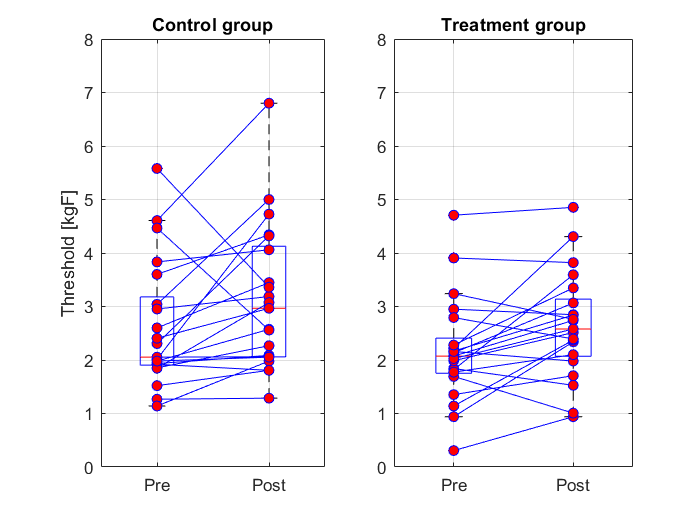
\includegraphics[width=1\textwidth]{figures/boxplot_threshold_all.PNG}  %<--but is not needed.
	\caption{}
	\label{fig:boxplot_thres_all}  %<--give the figure a label, so you can reference!
\end{figure}               %   For the label to work it must be under the caption.

Box plots showing the same for the tolerance is also made (figure \ref{fig:boxplot_tol_all}). 
\begin{figure}[H]                                         %   File-type can be specified
	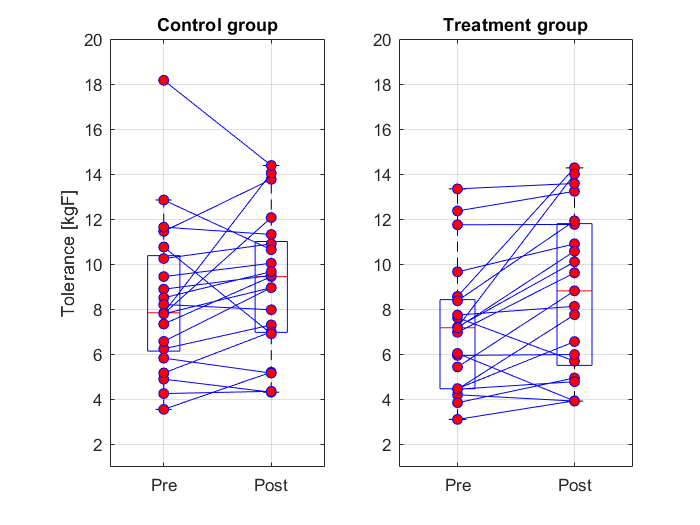
\includegraphics[width=1\textwidth]{figures/boxplot_tolerance_all.PNG}  %<--but is not needed.
	\caption{}
	\label{fig:boxplot_tol_all}  %<--give the figure a label, so you can reference!
\end{figure}               %   For the label to work it must be under the caption.

The mean percentage increase in the threshold and tolerance for the control and treatment are shown in figure \ref{fig:mean_increase_all}. 
 
\begin{figure}[H]                                         %   File-type can be specified
	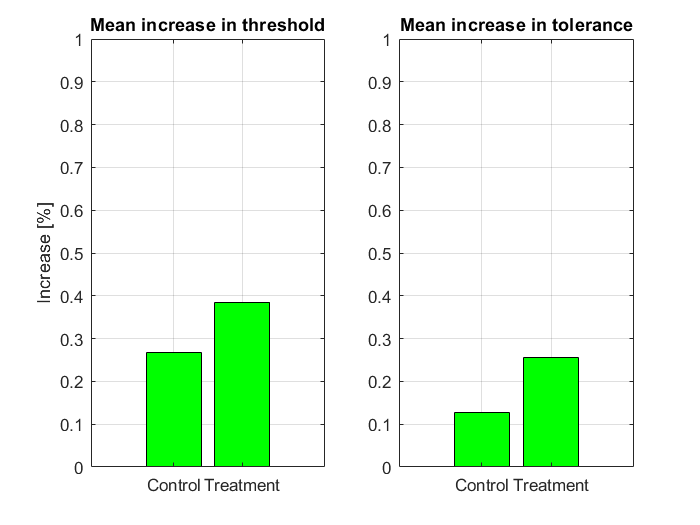
\includegraphics[width=1\textwidth]{figures/mean_increase_all.PNG}  %<--but is not needed.
	\caption{Mean percentage increase in threshold for control and treatment group (left) and mean percentage increase in tolerance for control and treatment group (right)}
	\label{fig:mean_increase_all}  %<--give the figure a label, so you can reference!
\end{figure}               %   For the label to work it must be under the caption.
